\section{Abstract Correlating Semantics}\seclabel{AbstractSem}

In this section, we introduce our correlating abstract domain which allows bounded representation of correlating program state while maintaining equivalence between correlated variables.

\subsection{Abstract Correlating State}

We represent variable information using standard relational abstract domains. As our analysis is path sensitive, we allow for a set of abstract sub-states, each adhering to a certain path in the product program. This abstraction is similar to the trace partitioning domain as described in~\cite{MauborgneRival07}.

%% EY: this is not a feature of the abstraction, it is a feature of the correlating program
%% the correlating program "assumes" that all correponding variables intially have the same value.
%To assure we only consider correlated paths from the product programs (starting from equivalent input states), our %abstraction will initially assume equality on all inputs.
Our power-set domain records precise state information but does not scale due to exponential blowup. As a first means of reducing state size, we define a special join operation that \emph{dynamically partitions} the abstract state according to the set of equivalences maintained in each sub-state and joins all sub-states in the same partition together (using the sub-domain join operation). This join criteria allows separation of equivalence preserving paths thus achieving better precision. Second, to allow a feasible bound abstraction for programs with infinite number of paths, we define a widening operator which utilizes the sub-domain's widening operator but cleverly chooses which sub-states are to be widened, according to path information encoded in state.
We start off by abstracting the correlating trace semantics in \ssecref{ConcreteCorrelatingSemantics}.

In the following, we assume an abstract relational domain $(\A{D}, \sqsubseteq_{D})$ equipped with operations $\sqcap_{D}$, $\sqcup_{D}$ and $\nabla_{D}$, for representing sets of concrete states in $\Sigma_{P \correlate P'}$. We separate the set of program variables into original program variables denoted $Var$ (which also include a special added variable for return value, if such exists) and the added guard variables denoted $Guard$ that are used for storing conditional values alone ($Guard$ also include a special added guard for return flag). We assume the abstract values in $\A{D}$ are constraints over the variables and guards (we denote $\A{D}_{Guard}$ for sub-domain abstraction of guards and $\A{D}_{Var}$ for original variables), and do not go into further details regarding the particular abstract domain as it is a parameter of the analysis. We also assume that the sub-domain $\A{D}$ allows for a sound over-approximation of the concrete semantics (given a sound interpretation of program operations). In our experiments, we use the polyhedra abstract domain~\cite{CousotHalbwachs78} and the octagon abstract domain~\cite{Mine2006}.

\begin{definition}[Correlating Abstract State] \deflabel{CorrelatingAbstractState}
A correlating abstract program state $\A{\sigma} \in Lab \rightarrow 2^{\A{D}_{Guard} \times \A{D}_{Var}}$, is a mapping from a correlating program label $l_{\correlate}$ to a set of pairs $(ctx, data)$, where $ctx \in \A{D}_{Guard}$ is the execution context i.e. an abstraction of guards values via the relational numerical domain and $data \in \A{D}_{Var}$ is an abstraction of the variables. \TODO{Should we explicitly say that Lab, Var, Guard denote correlating program labels, vars etc?}
\end{definition}

We separate abstractions over guard variables added by the transformation to GCL\footnote{Guarded command language} format (as defined in \secref{Correlating}) from original program variables as there need not be any relationships between guard and regular variables.

\subsection{Abstract Correlating Semantics}

\begin{table}
\footnotesize
\renewcommand{\arraystretch}{1.4}
\begin{tabular}{lcl}
\hline
$\asemp{v:=e}$ & \hspace{0.1in} & $l_{\correlate} \mapsto \{\langle ctx,\asemp{v:=e}_{\A{D}}(data) \rangle | \langle ctx,data \rangle \in S \}$
\\
\hline
$\asemp{g:=e}$ & & $l_{\correlate} \mapsto \{\langle \asemp{g:=true}_{\A{D}}(ctx),\asemp{e}_{\A{D}}(data) \rangle  | \langle ctx,data \rangle) \in S \}$ \\
& & ~~~~~~~~~~~$\cup \{ \langle \asemp{g:=false}_{\A{D}}(ctx),\asemp{\neg e}_{\A{D}}(data) \rangle | \langle ctx, data \rangle \in S \}$
\\ \hline
$\lsyn$ \textbf{if} (g) $\{s_{0}\}$ \textbf{else} $\{s_{1}\}$ $\rsyn^{\sharp}$ & &
$l_{\correlate} \mapsto \{\langle\asemp{g=true}_{\A{D}}(ctx),  \asemp{s_0}_{\A{D}}(data) \rangle | \langle ctx,data \rangle) \in S \}$ \\
& & ~~~~~~~~~~~$\cup \{\langle \asemp{g=false}_{\A{D}}(ctx), \asemp{s_1}_{\A{D}}(data) \rangle | \langle ctx,data \rangle \in S \}$
\\ \hline
$\lsyn$ \textbf{goto} lab $\rsyn^{\sharp}$ & & $\A{\sigma}$
\\ \hline
\end{tabular}
\renewcommand{\arraystretch}{1}
\caption{Abstract transformers}\label{Ta:AbsTrans}
\end{table}


\deflabel{CorrelatingAbstractSemantics}
\tabref{AbsTrans} describes the abstract transformers. The table shows the effect of each statement on a given abstract state $\A{\sigma} = l_{\correlate} \mapsto S$. The abstract transformers are defined using the abstract transformers of the underlying abstract domain $\A{D}$. We assume that any program $P$ can be transformed such that it only contains the operations described in \tabref{AbsTrans} (this is achieved by the GCL format). We also assume that for $\asemp{g:=e}$ operations, $e$ is a logical operation with binary value.

Next, we define the abstraction function $\alpha : 2^{\Sigma^{*}_{P \correlate P'}} \rightarrow 2^{\A{D} \times \A{D}}$ that abstracts together a set of concrete correlating traces $T$. As in our domain traces are abstracted together if they share the exact same path, we first define an operation $path : \Sigma^{*}_{P \correlate P'} \rightarrow Lab^{*}$ which returns a sequence of labels for a trace's states i.e. what is the path taken by that trace. We also allow applying $path$ on a set of traces to denote the set of paths resulting by applying the function of each of the traces. Finally we define the trace abstraction as following:
\[
\alpha(T) \triangleq \{ \sqcup_{path(\pi)=p} \beta(last(\pi)) | p \in path(T) \}
\]
where $\beta(\sigma) = \langle \beta_{\A{D}}(\sigma|_{Guard}), \beta_{\A{D}}(\sigma|_{Var}) \rangle$  i.e. applying the the abstraction function of the abstract sub-domain $\beta_{\A{D}}$ on parts of the concrete state applying to $Guards$ (denoted $\sigma|_{Guard}$) and $Vars$ (denoted $\sigma|_{Var}$) separately. Our abstraction partitions trace prefixes $\pi$ by path and abstracts together the concrete states reached by the prefix - $last(\pi)$, using the sub-domain.

%such that each $rd \in S_{RD}$ will abstract a certain \textbf{path} in the product program. We achieve that by instrumenting each $\sigma_{\times} = last(pre(\pi_{\times}))$ in the collecting semantics $CS(l_{\times})$ with the sequence of branches taken up to $\sigma_{\times}$ in $pre(\pi_{\times})$. This is easily achieved by using \emph{guard} values as they are recorded along the trace and we denote $path(\sigma_{\times})$ as the sequence of branches $b_0,...,b_n$ i.e. guard values ($b_i = <g,{T/F}>$), that led up to $\sigma_{\times}$. Therefore we define for every path $p_i$ in the product program the group of concrete correlating states that exist at the end of that path denoted $\Sigma_{\times}^{p_i} \triangleq \{ \sigma_{\times} | path(\sigma_{\times}) = p_i \}$. Finally we define the abstract state itself as $\C{\sigma_{\times}} \triangleq { rd | rd = ABS_{RD}(\Sigma_{\times}^{p_i}) \wedge p_i is a path in P \times P)}$. For example, the abstraction of \figref{MatchingProblemExamplePrograms}'s product program collecting semantics at labels $(lab,lab')$ will first collect together all trace prefixes that iterate the loop 0 times: $\Sigma_{\times}^{p_0} = \{  (x=0,i=0,x'=0,i'=0), (x=1,i=0,x'=1,i'=0), (x=2,i=0,x'=2,i'=0), ... \}$ and abstract them using the relational sub-domain to get $rd_{0} = \{x=x',i=i'=0\}$ which correctly expresses the fact that equivalence is kept in case none of the loops iterate. The next path to be abstracted would be where both loops iterate once i.e. $p_1 = <g,F>,<g',F>$ which also maintains equivalence and will be abstracted as $rd_{1} = \{x=x',i=i'=1, x \geq 1\}$. The next path however, which iterates the $P'$ loop twice but only once for the $P$ loop, $p_2 = <g,F>,<g',F>,<g,T>,<g',F>$ will not maintain equivalence as it will abstract $\Sigma_{\times}^{p_2} = \{  (x=1,i=1,x'=1,i'=2), (x=2,i=2,x'=2,i'=2), (x=3,i=2,x'=3,i'=2), ... \}$ as $rd_{2} = \{x=x',2 \leq i \geq 1, i'=2\}$. We mention that the abstract $rd$ ignores the separation of concrete states of $P$ and $P'$ and abstracts both variable data together. In fact, the ability to maintain direct relationships between the two sets of variables (and specifically those matched by $VC$) is crucial for maintaining equivalence.

Every path in the product program will be represented by a single sub-state of the sub-domain. As a result, all \emph{trace prefixes} that follow the same path to $l_{\correlate}$ will be abstracted into a single sub-state of the underlying domain. This abstraction fits semantics differencing well, as inputs that follow the same path display the same behavior and will usually either keep or break equivalence together, allowing us to separate them from other behaviors (it is possible for a path to display both behaviors as in \figref{PathProblemExamplePrograms} and we will discuss how we are able to manipulate the abstract state and separate equivalent behaviors from ones that offend equivalence). Another issue to be addressed is the fact that our state is still potentially unbound as the number of paths in the program may be exponential and even infinite (due to loops).

%\paragraph{Computing Abstract State with Our Analysis} \deflabel{ComputingAbstractState}
%We compute the correlating abstract state at each label $\C{\sigma_{\times}}$ by using means of abstract interpretation and program analysis. We interpret our correlating program (described in \secref{CorrelatingProgram}) which is a semantic preserving reduction over the much more arbitrary product program, using a standard fixed-point analysis algorithm, and apply interpreted operations on the set of sub-states of the current state $S_{RD}$. Our initial state explicitly assumes equality on all input variables (by adding a $v=v'$ constraint for every input variable $v$ where $v'=VC(v)$) to allow for sound checking of equivalence. This also allows for pruning of unfeasible paths where inputs diverge\COMMENT{ (though we may still interpret some as feasible due to incompleteness of program operations representation, for example bitwise operations)}. To adhere to the representation of traces in the abstract state, our join operation is in fact set union, thus indeed every prefix that reaches a certain program label will be awarded its own $rd$. Let us explicitly define the operations of the domain in our analysis:
%\begin{itemize}
%\item $S^{RD}_1 \sqsubseteq S^{RD}_2 \Longleftrightarrow \forall rd_1 \in G_1 \exists rd_2 \in G_2 : rd_1 \sqsubseteq_{RD} rd_2$
%\item $S^{RD}_1 \sqcap S^{RD}_2 \equiv { rd_1 \sqcap_{RD} rc_2 | rd_1 \in G_1 \wedge rd_2 \in G_2}$
%\item $S^{RD}_1 \sqcup S^{RD}_2 \equiv S^{RD}_1 \cup S^{RD}_2$
%\end{itemize}
%Next we define two more operations: Canonization (denoted $\odot$) - which allows for minimization of state size according to equivalence criteria and Widening (denoted $\nabla$) - which allows reaching a fixed-point when handling loops.

%\COMMENT{One advantage of our correlating domain over using two separate domains, is the ability to preserve equivalence in the face of non-linear operations - this argument may be too thin to include.}

\begin{figure}
\centering
\begin{tabular}{cc}
\begin{lstlisting}
int f(int x) {
    return x;
}
\end{lstlisting}
\hspace{1cm}
&
\begin{lstlisting}
int f'(int x) {
    return 2*x;
}
\end{lstlisting}
\end{tabular}
\caption{Single path differentiation candidates}
\figlabel{PathProblemExamplePrograms}
\end{figure}


\subsection{Dynamic Partitioning}

Performing analysis with the powerset domain does not scale as the number of paths in the correlated program may be exponential (we defer the case of unbound paths to widening of loops). We must allow for reduction of state $\A{\sigma} = l_{\correlate} \mapsto S$ with acceptable loss of precision. This reduction via partitioning can be achieved by joining the abstract sub-states in $S$ (using the standard join of the sub-domain). However this can only be accomplished after first deciding which of the sub-states shall be joined together and then choosing the program locations for the partitioning to occur. In order to choose a strategy, we start by taking a closer look at the final state of the fully disjunctive analysis of \figref{SignCorrelating}:
{\footnotesize
\[
\A{\sigma}(end) = [ \langle (g1,\neg g2',\equiv_{g1}),(x>0,sgn=1,\equiv_{x,sgn}) \rangle,
\]
\[
\langle (\neg g1,\neg g2',\equiv_{g1}), (x<0,sgn=-1,\equiv_{x,sgn}) \rangle,
\langle (\neg g1,g2',\equiv_{g1}),(x=0,sgn=0,sgn'=1,\equiv_{x}) \rangle ]
\]
}
One may observe that were we to join the two sub-states that maintain equivalence on $\{x,sgn,g1\}$, it would result in an acceptable loss of precision (losing the $x$ related constraints). This is achieved by partitioning sub-states according to \emph{the set of variables which they preserve equivalence for}. This bounds the state size at $2^{|VC|}$, where $VC$ is the set of correlating variables we wish to track.
As mentioned, another key factor in preserving equivalence and maintaining precision is the program location at which the partitioning occurs. The first possibility, which is somewhat symmetric to the first proposed partitioning strategy, is to partition at every join point i.e. after every branch converges. Let use examine $sign \bowtie sign'$ state after processing the first guarded instruction \scode{if (g1) sgn = -1;} (we ignored $g2'$ effect at this point for brevity):
{\footnotesize
\[
\A{\sigma} = [ \langle (g1,\equiv_{g1}),(x \geq 0,\equiv_{x,sgn}) \rangle,
\langle (g1,\equiv_{g1}),(x < 0,sgn' = -1, \equiv_{x}) \rangle ]
\]
}
This suggests that partitioning at join points will perform badly in many scenarios, specifically here as we will lose all data regarding $sgn$. However if we could delay the partitioning to a point where the two programs ''converge'' (after the following \scode{if (g1') sgn' = -1;} line), we will get a more precise temporary result which preserves equivalence. To accomplish this, we define special program locations we name \emph{correlating points} which present places where programs have likely converged. These are a sub-product of the correlating program construction process described in \secref{Correlating}.

%We can see from our motivating example that it is not feasible to allow our correlating domain to keep diverging and double in size with every conditional as it will exponentially blow up the analysis run-time and memory. Instead, we employ an equivalence conserving canonization technique such that at every canonization point we will partition the sub-states according to the set of variables to which they hold equivalence for and join these all together into one abstract, using the sub-domain lossy join. This bounds the number of abstracts in the state to $2^{|V|}$ for variables correlated $VC$. This fine grained equivalence checking is successful in telling apart paths that hold equality for none, some or all of the variables. For instance in \figref{MatchingProblemExamplePrograms}, our canonization will tell apart the sub-state that hold equivalence for all variables $\{i=i'=x=x'=0\}$ from the rest that hold equivalence for $x$ alone and join them all together into the $\{x=x',i \leq x, i' \leq 2x'\}$ state. The fact that we did not lose equivalence altogether is beneficial as we are able to report that the input variable $x$ did not diverge which may be of use in case \scode{foo} had used $x$ further down the road.

\begin{figure}
\centering
\begin{tabular}{c}
\begin{lstlisting}
unsigned max = ...;
int sum''(int arr[], unsigned len) {
  int result = 0;
  if (len > max)
    return -1;
  for (unsigned i = 1; i < len; i+=2)
    result += arr[i];
 return result;
}
\end{lstlisting}
\\
\\ \hline
\\
\begin{lstlisting}
unsigned max' = ...;
int sum(int arr[], unsigned len) {
  unsigned len' = len;
  int arr'[] = arr;
  int result = 0;
  int result' = 0;
  guard r' = (len' > max');
  if (r') retval' = -1;
  if (r') r' = 0;
  {
    unsigned i = 1;
    unsigned i' = 1;
l:  guard g = (i < len);
l': guard g' = (i' < len');
    if (g) result += arr[i];
    if (r') if (g') result' += arr'[i'];
    if (g) i+=2;
    if (r') if (g') i'+=2;
    if (g) goto l;
    if (r') if (g') goto l';
  }
}
\end{lstlisting}
\end{tabular}
\caption{Patched $sum'$ and correlating $sum \bowtie sum''$}
\figlabel{LoopCorrelatingExample2}
\end{figure} 

\subsection{Widening}

In order for our analysis to handle loops we require a means for reaching a fixed point. As our analysis iterates over a loop, sub-states may be added or transformed continuously, never converging. We therefore need to define a widening operator for our new domain, which will further over-approximate the looping state and arrive at a fixed point. We have the widening operator of our sub-domain at our disposal, but we are faced with the question of how to apply this operator, i.e. which pairs of sub-states $\langle ctx , data \rangle$ from $\A{\sigma}$ should be widened with which. A first viable strategy is to perform an overall join operation on all pairs which will result in a single pair of sub-states and then simply apply the widening to this sub-state using the sub-domain's $\nabla$ operator. If we examine applying this strategy to $sum \bowtie sum'$ from \figref{LoopCorrelatingExample}, we get that it will successfully arrive at a fixed point that also maintains equivalence as all sub-states maintain equivalence at loop back-edges. Now let us try to apply the strategy to the more complex $sum \bowtie sum''$ as seen in \figref{LoopCorrelatingExample2}. First we mention that as $sum'$ introduces a return statement under the $len > max$ condition, the example shows an extra $r'$ guard and $retval'$ variable for representing a return (this exists in all GCL programs but we omitted it so far for brevity). While analyzing, once we pass that first conditional, our state is split to reflect the return effect:
{\footnotesize
\[
\A{\sigma} = [ d_1 = \langle (\neg r'),(len \leq max, result = 0, \equiv_{len,result}) \rangle,
\]
\[
d_2 = \langle (r'),(len > max, retval' = -1, result = 0, \equiv_{len,result}) \rangle ]
\]
}
As we further advance into the loop, $d_1$ will maintain equivalence but $d_2$ will continue to update the part of the state regarding untagged variables  (since $r'$ is $false$), specifically it will change $result$ continuously, preventing the analysis from reaching fixed point. We would require widening here but using the naive strategy of a complete join will result in aggressive loss of precision, specifically losing all information regarding $result$. The problem originates from the fact that prior to widening, we joined sub-states which adhere to two different loop behaviors: one where both $sum$ and $sum'$ loop together (that originated from $len < max$) and the other where $sum'$ has exited but $sum$ continues to loop ($len \geq max$). Ideally, we would like to match these two behaviors and widen them accordingly. We devised a widening strategy that allows us to do this as it basically matches sub-states that adhere to the same behavior, or loop-paths. This strategy dictates using \emph{guards} for the matching. If two sub-states agree on their set of guards, it means they represent the same loop path and can be widened as the latter originated from the former (widening operates on subsequent iterations). In our example, using this strategy will allow the correct matching of states after consequent $k, k+1$ loop iterations:
{\footnotesize
\[
\A{\sigma}_{k} = [ d_1 = \langle (\neg r',g,\equiv_{g}),(len \leq max, i = 2k + 1, \equiv_{i,len,result}) \rangle,
\]
\[
d_2 = \langle (r',\neg g,g'),
(len > max, retval' = -1, result' = 0, i' = 2k + 1, i = 1, \equiv_{len}) \rangle ]
\]
}
{\footnotesize
And:
\[
\A{\sigma}_{k+1} = [ d_1 = \langle (\neg r',g,\equiv_{g}),(len \leq max, i = 2k + 3, \equiv_{i,len,result}) \rangle,
\]
\[
d_2 = \langle (r',\neg g,g'),
(len > max, retval' = -1, result' = 0, i' = 2k + 3, i = 1, \equiv_{len}) \rangle ]
\]
}
As we can identify the states predecessors by simply matching the guards. $d_1$ will be widened for a precise description of the difference shown as $\langle len = len' > max', retval' = -1, retval = \top \rangle$.

\subsection{Differencing for Abstract Correlating States} \sseclabel{CorrelatingAbstractDiff}
\TODO{Maybe move this entire part to an appendix, or at least the algorithm part.}\\
Given an abstract state in our correlating domain, we want to determine whether equivalence is kept and if so under which conditions it is kept (for partial equivalence) or determine there is difference and characterize it. As our state may hold several pairs of sub-states, each holding different equivalence data, we can provide a verbose answer regarding whether equivalence holds. We partition our sub-states according to the set of variables they hold equivalence for and report the state for each equivalence partition class. Since we instrument our correlating program to preserve initial input values, for some of these states we will also be able to report input constraints thus informing the user of the input ranges that maintain equivalence. When equivalence could not be proved, we report the offending states and apply a differencing algorithm for extracting of the delta. \figref{PathProblemExamplePrograms} shows an example of where our analysis is unable to prove equivalence, although part of the state does maintain equivalence (specifically for $x=0$). This is due to the abstraction being too coarse. We describe an algorithm that given a sub-state $d \in \A{D}$, computes the differentiating part of the sub-state (where correlated variables disagree on values) by splitting it into parts according to equivalence. This is done by treating the relational constraints in our domain as geometrical objects and formulating delta based on that.

%\para{Correlating Abstract State Delta}
\begin{definition} [Correlating Abstract State Delta] \deflabel{CorrelatingAbstractStateDelta}
Given a sub-state $d$ and a correspondence $VC$, the correlating state delta $\triangle_{A}(d)$, computes abstract state differentiation over $d$. The result is an abstract state $\sqsubseteq d$ approximating all concrete values for variables correlated by $VC$, that differ between $P$ and $P'$. Formally, the delta is simply the abstraction of the concrete trace deltas:
\[
\triangle_{A}(d)^{+} \triangleq \alpha(\cup_{path}\triangle_{T}^{+}) ,
\triangle_{A}(d)^{-} \triangleq \alpha(\cup_{path}\triangle_{T}^{-})
\]
where deltas are grouped together by path and then abstracted.
\end{definition}
The algorithm for the extraction of delta from a correlating state, is as follows:
\begin{enumerate}
\item $d_{\equiv}$ is a state abstracting the concrete states \emph{shared} by the original and patched program. It is achieved by computing: $d_{\equiv} \triangleq d|_{V=V'} \equiv d \sqcap \bigwedge\{ v = v' | (v,v') \in VC \}$.
\item $\overline{d_{\equiv}}$ is the negated state i.e. $\A{D} \setminus d_{\equiv}$ and it is computed by negating $d_{\equiv}$ (as mentioned before, all logical operations, including negation, are defined on our representation of an abstract state).
\item Eventually: $\triangle_{A}(d) \triangleq d \sqcap \overline{d_{\equiv}}$ abstracts all states in $P \times P'$ where correlated variables values do not match.
\item $\triangle_{A}(d)^{+} = \triangle_{A}(d)|_{V'}$ is a projection of the differentiation to display values of $P'$ alone i.e. "added values".
\item $\triangle_{A}(d)^{-} = \triangle_{A}(d)|_{V}$ is a projection of the differentiation to display values of $P$ alone i.e. "removed values".
\end{enumerate}
\begin{Example}
Applying the algorithm on \figref{PathProblemExamplePrograms}'s $P$ and $P'$ where $d = \{ retval' = 2retval \}$ will result in the following:
\begin{enumerate}
\item $d_{\equiv} = \langle retval' = 0, retval = 0 \rangle$.
\item $\overline{d_{\equiv}} = [ \langle retval' > 0 \rangle, \langle retval' < 0 \rangle, \langle retval > 0 \rangle, \langle retval < 0 \rangle ]$
\item $\triangle_{A}(d)  = [ \langle retval' = 2retval, retval' > 0 \rangle, \langle retval' = 2retval, retval' < 0 \rangle, \langle retval' = 2retval, retval > 0 \rangle, \langle retval' = 2retval, retval < 0 \rangle ]$
\item $\triangle_{A}(d)^{+} = [ \langle retval' > 0 \rangle, \langle retval' < 0 \rangle ]$
\item $\triangle_{A}(d)^{-} = [\langle retval > 0 \rangle, \langle retval < 0 \rangle]$
\end{enumerate}
\end{Example}
We note that as a sub-state is basically a conjunction of constraints, negating it by splitting to constraints and negating each individually reflects correctly the effect of negating a conjunction as we are left with a disjunction of negations, as seen in step 2.
We also see that displaying the result in the form of projections is ill-advised as in some states differentiation data is represented by relationships on correlated variables alone, thus projecting will lose all data and we will be left with a less informative result. A geometrical representation of $\triangle_{A}$ calculation can be seen in \figref{Delta}.

\begin{figure}
\centering
\begin{tabular}{c}
\imagetop{
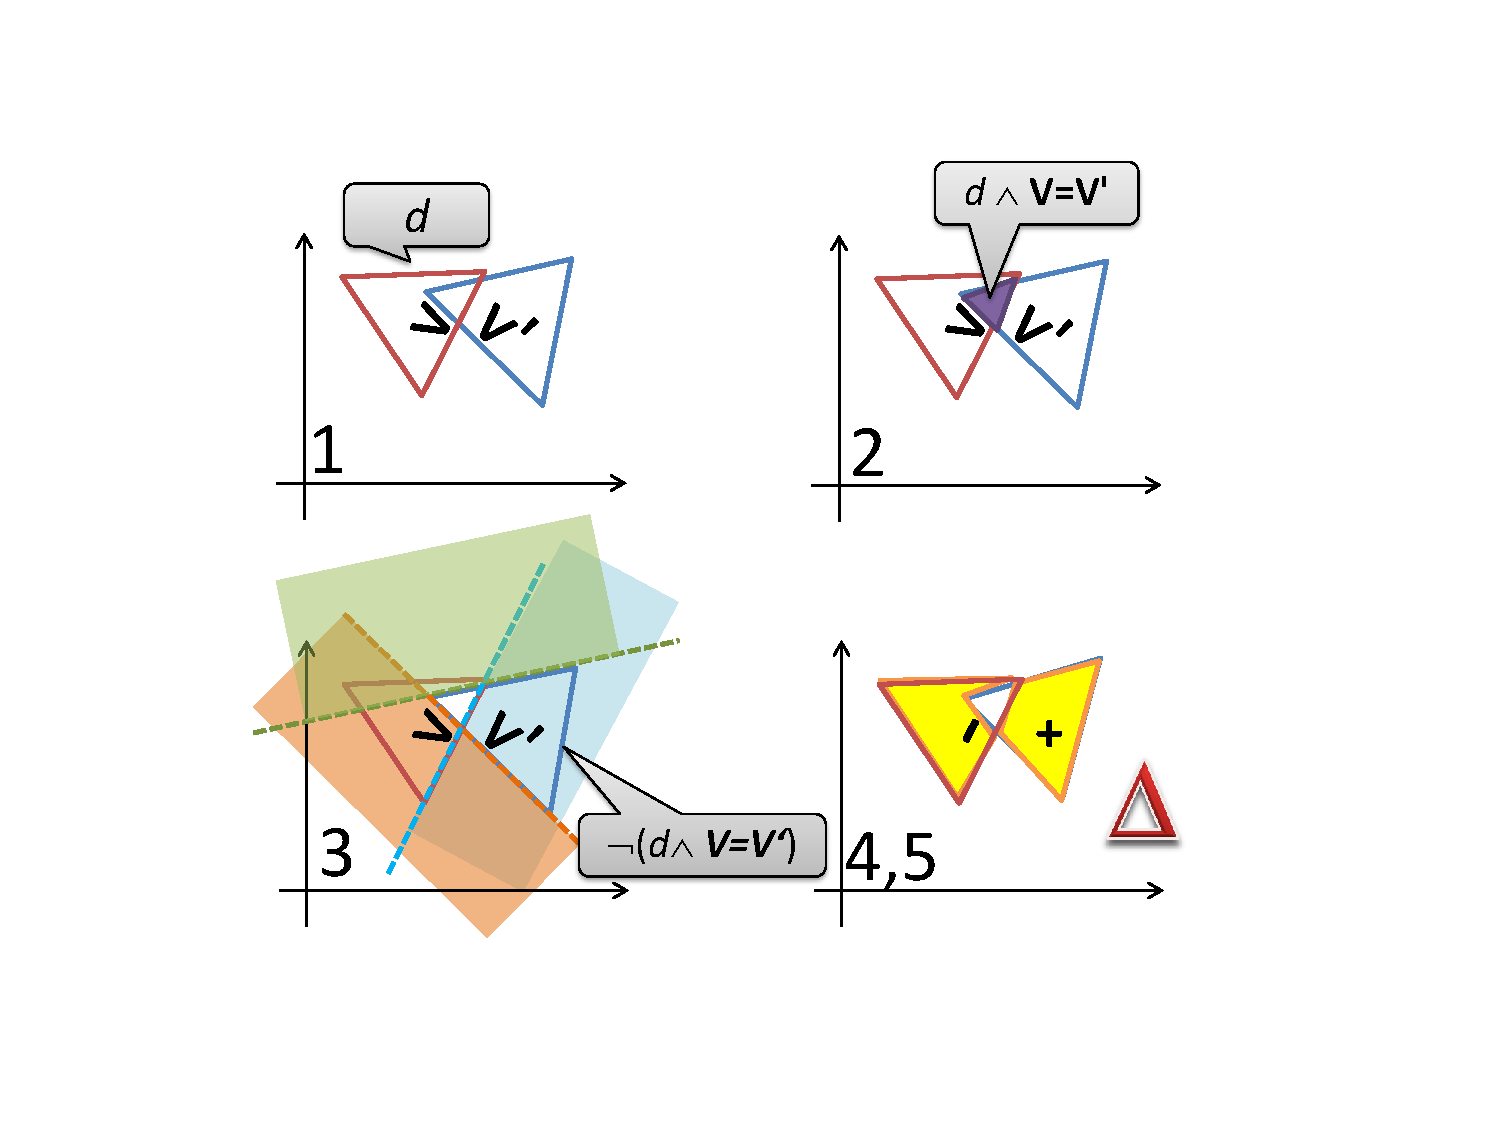
\includegraphics[scale=0.45,clip=true,trim = 125pt 75pt 150pt 75pt]{figures/delta}
}
\end{tabular}
\caption{Delta computation geometrical representation.}\figlabel{Delta}
\end{figure}

%\begin{algorithm}
\small
\DontPrintSemicolon
%\linesnumbered
\SetAlgoLined
\SetAlgoSkip{bigskip}
\KwIn{Abstract state $rd$}
\KwOut{Abstract difference - $\triangle(rd)$}
$rd_{\equiv} \leftarrow rd \sqcap \bigwedge\{ v = v' | VC(v) = v'\}$\;
$\overline{rd_{\equiv}} \leftarrow \neg rd_{\equiv} = \{ \neg c | c \in rd_{\equiv}\}$\;
Foreach $rd_i \in \overline{rd_{\equiv}}$:
    $\triangle(rd) \leftarrow \triangle(rd) \cup (rd \sqcap rd_i$)\;
\Return $\triangle(rd)$
\caption{Compute Abstract Difference.}\label{Alg:AbsDiff}
\end{algorithm}
%% RESET THE ALGORITHMS COUNTER TO PUSHBACK INC FROM FUNCTIONS
\setcounter{algocf}{1}


From this point forward any mention of 'delta' (denoted $\triangle$) will refer to the correlating abstract state delta (denoted $\triangle_{A})$. We claim that $\triangle$ is a correct abstraction for the concrete state delta which allows for a scalable representation of difference we aim to capture.
